\section{What is a Function?}
\label{sec:functions}
% To do: graphs, images, Excel/LibreOffice Calc spreadsheets.

\subsection{Function Concepts}

The natural world is full of relationships between quantities that change. When we see these
relationships, it is natural for us to ask ``If I know one quantity, can I then determine the other?" This establishes the idea of an input quantity, or {\bf independent variable}\index{Variable!independent}, and a corresponding output quantity, or {\bf dependent variable}\index{Variable!dependent}. From this, we get the notion of a functional relationship in which the output can be determined from the input.

For some quantities, like height and age, there are certainly relationships between these
quantities. Given a specific person and any age, it is easy enough to determine their height, but if we tried to reverse that relationship and determine age from a given height, that would be problematic, since most people maintain the same height for many years.

\begin{definition}
A {\bf function}\index{Function} is a rule for a relationship between an {\bf input} (or {\bf independent}) quantity and an {\bf output} (or {\bf dependent}) quantity in which each input value uniquely determines one output value. We say ``the output is a function of the input."
\end{definition}

\begin{example}
\label{ex:height}
In the height and age example above, is height a function of age? Is age a function of height?

\begin{solution} In the height and age example above, it would be correct to say that height is a function of age, since each age uniquely determines a height. You cannot have two different heights at any one instant in time.

However, age is not a function of height, since one height input might correspond with more than one output age. Once you have stopped growing, your height essentially remains constant for the rest of your life.
\end{solution}\end{example}

\subsection{Representing Functions}

Functions can be represented in many ways:
    \begin{multicols}{2}
    \begin{enumerate}
        \item A description of a relationship between variables,
        \item Tables of values,
        \item Graphs,
        \item Formulas,
        \item An action verb, and
        \item A black box with input and output.
    \end{enumerate}
    \end{multicols}
Example \ref{ex:height} represented a function in words, but it will be convenient to streamline the discussion of a function. To that end, we introduce notation of functions.

\paragraph{Function Notation.}

To simplify writing out expressions and equations involving functions, a simplified notation is often used. We also use descriptive variables to help us remember the meaning of the quantities in the problem.

Rather than write ``height is a function of age'', we could use the descriptive variable $h$ to represent height and we could use the descriptive variable $a$ to represent age.

If we name the function $f$ we could write ``height is a function of age" as ``$h$ is $f$ of $a$," or more simply:
$$h = f(a) \enspace .$$

We could instead name the function $h$ and write $h(a)$, which is read ``$h$ of $a$."

We can use any variable to name the function; the notation $h(a)$ shows us that $h$ depends on $a$. The value ``$a$'' must be put into the function ``$h$'' to get a result.

\begin{remark}
Be careful! The parentheses indicate that age is the input into the function. Do not confuse these parentheses with multiplication!
\end{remark}

\begin{example}
A function $N = f(y)$ gives the number of police officers, $N$, in a town in year $y$. What does $f(2005) = 300$ tell us?

\begin{solution} When we read $f(2005) = 300$, we see the input quantity is 2005, which is a value for the input quantity of the function: the year ($y$). The output value is $300$, the number of police officers ($N$), a value for the output quantity. Remember $N=f(y)$. This tells us that in the year 2005 there were 300 police officers in the town.
\end{solution}\end{example}

\paragraph{Tables as Functions.}

A table lists the input and corresponding output values of a function.

In some cases, these values represent everything we know about the relationship, while in other cases the table is simply providing us a few select values from a more complete relationship.

Table \ref{tab:function} below represents the age of a child in years and his
corresponding height. This represents just some of the data available
for the age and height of the child.

\begin{table}[ht!]
\begin{centering}
\begin{tabular}{l*{7}{r}}
\toprule
{\bf (Input:)} $a$, age (years) & 4 & 5 & 6 & 7 & 8 & 9 & 10\\
\midrule
{\bf (Output:)} $h$, height (inches) & 40 & 42 & 44 & 47 & 50 & 52 & 54\\
\bottomrule
\end{tabular}
\caption{Tabulating height as a function of age for a child.}
\label{tab:function}
\end{centering}
\end{table}
From this, we can create equations such as $h(6) = 44$, meaning that when the child was 6 years old, he was 44 inches tall.


\begin{example}

Which of these tables define a function (if any)?

\begin{center}
\begin{tabular}{ccc}
\multicolumn{2}{c}{Table A.}\\
\toprule
{\bf Input} & {\bf Output}\\
\toprule
2 & 1 \\
\midrule
5 & 3 \\
\midrule
8 & 6 \\
\bottomrule
\end{tabular}
\quad
\begin{tabular}{ccc}
\multicolumn{2}{c}{Table B.}\\
\toprule
{\bf Input} & {\bf Output}\\
\toprule
$-3$ & 5 \\
\midrule
0 & 1 \\
\midrule
4 & 5 \\
\bottomrule
\end{tabular}
\quad
\begin{tabular}{ccc}
\multicolumn{2}{c}{Table C.}\\
\toprule
{\bf Input} & {\bf Output}\\
\toprule
1 & 0 \\
\midrule
5 & 2 \\
\midrule
5 & 4 \\
\bottomrule
\end{tabular}
\end{center}

\begin{solution} Tables A and B define functions. In both tables, each input corresponds to exactly one output. Table C does not define a function since the input value of 5 corresponds with two different
output values: 2 and 4.
\end{solution}\end{example}



\paragraph{Graphs as Functions}

A function can often be represented as a {\bf graph}\index{Graph}, a set of {\bf points}\index{Point} plotted on {\bf coordinate axes}\index{Coordinate axes}: the {\bf horizontal axis}\index{Axis!horizontal} and the {\bf vertical axis}\index{Axis!vertical}. By convention, graphs are typically created with the input quantity along the horizontal axis and the output quantity along the vertical axis.

Points on the graph are represented by ordered pairs of the form $(a, b)$. Beginning at the {\bf origin}\index{Origin} (the point $(0,0)$), you move $a$ units to the left and $b$ units up to arrive at the point $(a, b)$. If $a<0$, then movement is to the left and if $b<0$, then movement is down.

\begin{wrapfigure}{r}{0.3\textwidth}
    \centering
    \vspace{-12pt}
    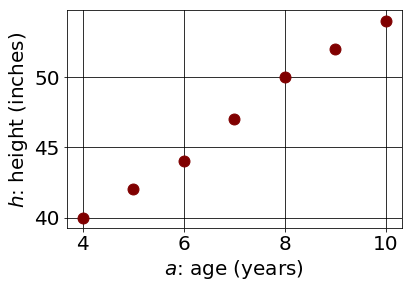
\includegraphics[width=0.3\textwidth]{img/chap1/sec1-2/table1-1.png}\\
    \caption{A plot of height data.}
    \label{fig:heightplot}
\end{wrapfigure}
The horizontal and vertical axes are typically called the {\bf $x$-axis}\index{$x$-axis} and the {\bf $y$-axis}\index{$y$-axis}, but these axes can be labeled with any variable name, not just $x$ and $y$. We say $y$ is a function of $x$, or $y = f(x)$ when the function is named $f$. The point $(a, b)$ lies on the graph of the function $f$ if and only if $f(a)=b$.

As an example, Figure \ref{fig:heightplot} is a plot of the data from Table \ref{tab:function}.

\begin{example}
\label{ex:1-2-graphs}
Which of these graphs defines a function $y=f(x)$?
\begin{figure}[!ht]
    \centering
    \begin{subfigure}[b]{0.3\textwidth}
        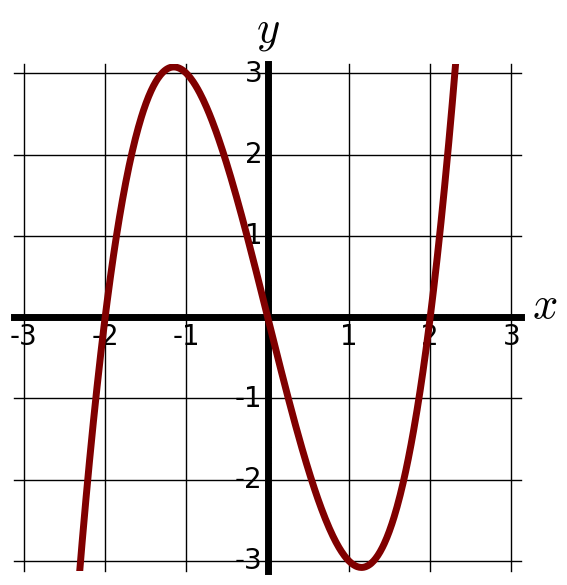
\includegraphics[width=\textwidth]{img/chap1/sec1-2/ex114a.png}
        \caption{Graph A}
    \end{subfigure}
    ~
    \begin{subfigure}[b]{0.3\textwidth}
        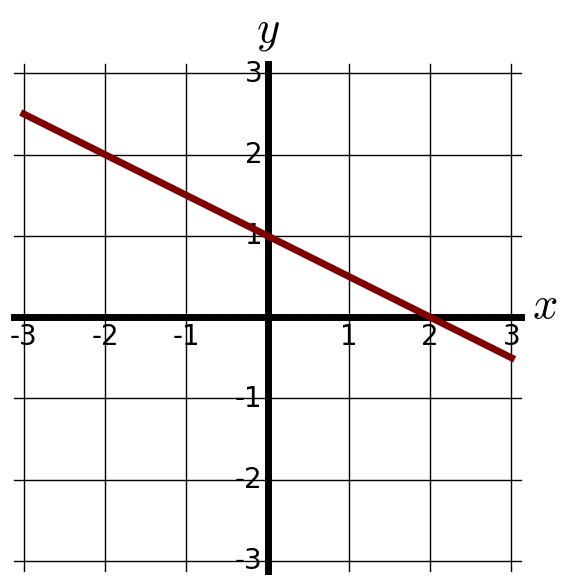
\includegraphics[width=\textwidth]{img/chap1/sec1-2/ex114b.png}
        \caption{Graph B}
    \end{subfigure}
    ~
    \begin{subfigure}[b]{0.3\textwidth}
        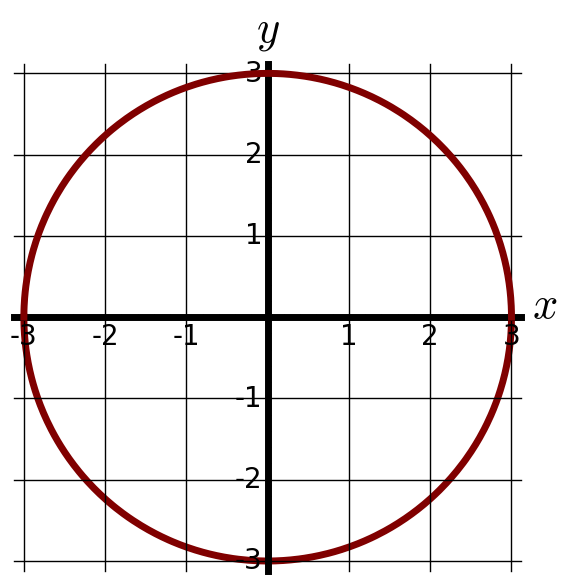
\includegraphics[width=\textwidth]{img/chap1/sec1-2/ex114c.png}
        \caption{Graph C}
    \end{subfigure}
\end{figure}

\begin{solution} Looking at the graphs above, Graphs A and B define a function $y=f(x)$, since for each input value along the horizontal ($x$) axis, there is exactly one corresponding output value, determined by the $y$-value of the graph. Graph C does not define a function $y=f(x)$ since some input values, such as
$x=2$, correspond with more than one output value.
\end{solution}\end{example}

\begin{wrapfigure}{r}{0.3\textwidth}
    \centering
    \vspace{-12pt}
    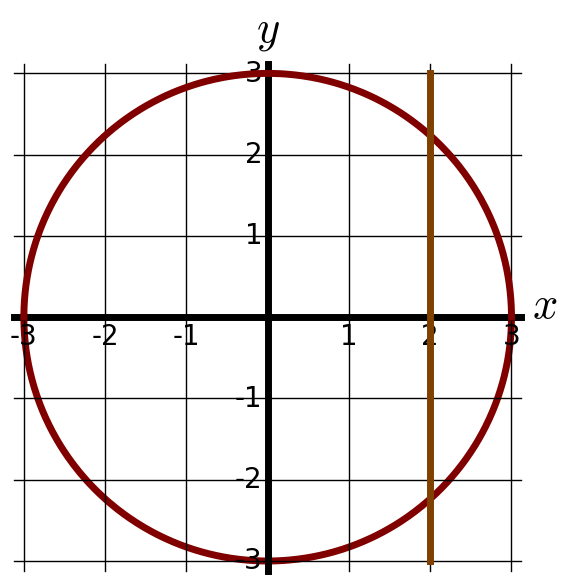
\includegraphics[width=0.3\textwidth]{img/chap1/sec1-2/fig115.png}\\
    \caption{A graph failing the vertical line test.}
    \label{fig:1-2-115}
\end{wrapfigure}
The \textbf{vertical line test}\index{Vertical line test} is an easy way to determine whether a graph defines a function or not. Imagine drawing vertical lines through the graph. Since a function has exactly one output for every input, if there is a vertical line that would cross the graph more than once, then the graph does not define a function.

Figure \ref{fig:1-2-115} illustrates how Graph C from Example \ref{ex:1-2-graphs} fails the vertical line test. The vertical line $x=2$ (in gold) intersects Graph C (in maroon) at two points; there are two outputs for for the input $x=2$.

\paragraph{Formulas as Functions}

When possible, it is very convenient to define relationships between quantities using a formula. If it is possible to express the output as a formula involving the input quantity, then we can define a function.

\begin{example}
Express the relationship $2N + 6p = 12$ as a function $p = f(N)$ if possible.

\begin{solution} To express the relationship in this form, we need to be able to write
the relationship where $p$ is a function of $N$, which means
writing it as $p = $ something involving $N$, or $p$ in terms of $N$. We proceed using algebra.

\begin{align*}
&2N + 6p = 12& &\mbox{Subtract $2N$ from both sides.}\\
&6p = 12 - 2N& &\mbox{Divide both sides by 6 and simplify.}\\
&p = \frac{12-2N}{6}& & \\
&p = \frac{12}{6} - \frac{2N}{6} & &\\
&p = 2 - \frac{1}{3}N & &
\end{align*}
We can now express $p$ as a function of $N$:
$$p = f(N) = 2 - \frac{1}{3}N \enspace .$$
\end{solution}\end{example}

It is important to note that not every relationship can be expressed as a function with a formula. Consider the examples of the boy's height as a function of age in Table \ref{tab:function} or a company's stock price as a function of time. Neither situation allows one to define the relationship using a formula precisely, yet we still may want to analyze aspects of these relationships using tools of calculus. The rest of the chapter will introduce us to some tools to help us with that.

Note the important feature of an equation written as a function is that the output value can be determined directly from the input by doing evaluations. This allows the relationship to act as a magic box that takes an input, processes it, and returns an output. Modern technology and computers rely on these functional relationships, since the evaluation of the function can be programmed.

\subsection{Evaluating Functions.}

The fundamental use of a function is to {\bf evaluate} the function: ``plugging in" some number into the function, or more precisely, to determine the corresponding output for a given input. In other words, we substitute or replace the input variable of the function with the input value. Evaluating will always produce one result, since each input of a function corresponds to exactly one output. We can evaluate a function from a table, graph, or formula.

Another related use is to determine the input or inputs of a function, given an output of the function. This is called {\bf solving} an equation and could produce more than one solution, since different inputs can produce the same output.

\begin{remark}
The concepts of evaluating and solving often get confused. When we use the word {\em solve}, we will be {\em solving a problem} or {\em solving an equation for an unknown quantity or variable}. It does not make sense to solve a function, since a function is merely a mathematical expression and not an equation.
\end{remark}

\begin{example}
Let $Q=g(n)$ and use the table shown.

\begin{center}
    \begin{tabular}{*{6}{l}}
    \multicolumn{6}{c}{$Q = g(n)$ as a table.}\tabularnewline
    \toprule
    $n$ & 1 & 2 & 3 & 4 & 5 \tabularnewline
    \midrule
    $Q$ & 8 & 6 & 7 & 6 & 8 \tabularnewline
    \bottomrule
    \end{tabular}
\end{center}

    \begin{itemize}
        \item[(a)] Evaluate $g(3)$.

\begin{solution} Evaluating $g(3)$, read ``$g$ of 3,'' means that we need to determine the output value, $Q$, of the function $g$ given the input value of $n=3$. Looking at the table, we see the output corresponding to $n=3$ is $Q=7$, allowing us to conclude $g(3) = 7$.
\end{solution}
    \item[(b)] Solve $g(n) = 6$ for $n$.

    \begin{solution} Solving $g(n) = 6$ means we need to determine what input values, $n$, produce an output value of 6. Looking at the table we see there are two solutions: $n = 2$ and $n = 4$.

      When we evaluate $g(n)$ at 2, our output is $Q = 6$.

      When we evaluate $g(n)$ at 4, our output is also $Q= 6$.
    \end{solution}
    \end{itemize}
\end{example}

Evaluating a function using a graph requires taking the given input and using the graph to look up the corresponding output. Solving a function equation using a graph requires taking the given output and looking on the graph to determine the corresponding input.

\begin{minipage}{0.65\textwidth}
\begin{example}
Consider the graph of a function $f(x)$ to the right.

    \begin{itemize}

        \item[(a)] Evaluate $f(2)$.

        \begin{solution} To evaluate $f(2)$, we find the input of $x=2$ on the horizontal ($x$) axis. Moving up to the graph gives the point $(2, 1)$, giving an output of $y=1$. Therefore, $f(2) = 1$.
\end{solution}
        \item[(b)] Solve $f(x) = 4$ for $x$.

        \begin{solution} To solve $f(x) = 4$, we find the value 4 on the vertical ($y$) axis because if $f(x) = 4$ then 4 is the output. Moving horizontally across the graph gives two points with the output of 4: $(-1,4)$ and $(3,4)$. These give the two solutions to $f(x) = 4$: $x = -1$ or $x = 3$.

        This means $f(-1)=4$ and $f(3)=4$, or when the input is $-1$ or 3, the output is 4.
        \end{solution}
    \end{itemize}

\end{example}
 \end{minipage}
 \begin{minipage}{0.3\textwidth}
%\begin{figure}
 %{wrapfigure}{r}{0.3\textwidth}
 %\begin{floatingfigure}{0.3\textwidth}
%     \centering
     %\vspace{-32pt}
     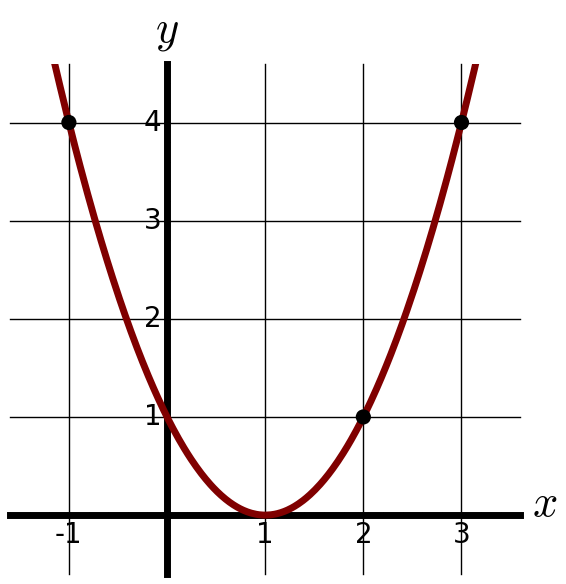
\includegraphics[width=\textwidth]{img/chap1/sec1-2/ex117.png}
 %\end{wrapfigure}
 %\end{floatingfigure}
%\end{figure}
\end{minipage}

\begin{example}
Let $k(t) = t^3 + 2$.
    \begin{itemize}
        \item[(a)] Evaluate $k(2)$.

        \begin{solution} To evaluate $k(2)$, we replace $t$ with 2 in the expression $t^3+2$, then simplify.
        \begin{align*}
            k(2) &= 2^3 + 2 \\
            &= 8 + 2 \\
            &= 10
        \end{align*}
        So $k(2) = 10$.
        \end{solution}
        \item[(b)] Solve $k(t) = 1$ for $t$.

        \begin{solution} To solve $k(t) = 1$, we set the formula for $k(t)$ equal to 1, and solve for the input value that will produce that output.
        \begin{align*}
            k(t)    &=  1 & &\mbox{Substitute the original formula } k(t) = t^3 + 2.\\
            t^3 + 2 &=  1 & &\mbox{Subtract 2 from each side}. \\
            t^3     &= -1 & &\mbox{Evaluate the cube root of each side.}\\
            t       &= \sqrt[3]{-1} = -1& &
        \end{align*}

When solving an equation using formulas, you can check your answer by using your solution in the original equation to see if your calculated answer is correct.

To check our work, we want to know if $k(t)=1$ is a true statement when $t=-1$.
    \begin{align*}
        k(-1) &= (-1)^3 + 2 \\
              &= -1 + 2 \\
              &= 1 \enspace ,
          \end{align*}
which was the desired result.
\end{solution}
    \end{itemize}
\end{example}


\subsection{Cost, Revenue, Profit, and Demand}
\label{ssec:cost}
Suppose that your club wants to raise funds by selling T-shirts. The screen printing shop that will make the shirts will charge your club \$50 to cover overhead costs and \$5 per shirt for the shirts themselves. You decide to charge \$15 per shirt. Some questions naturally arise. How many shirts need to be sold to {\bf break even}? How much {\bf profit} can be expected?

We can describe situations such as this with functions. The {\bf total cost}\index{Cost!total} to produce these shirts combines {\bf fixed costs}\index{Cost!fixed} and {\bf variable costs}\index{Cost!variable}. The fixed costs are also called {\bf overhead costs} and do not depend on the number of T-shirts made, while the variable costs are the per item cost. If $n$ is the number of T-shirts the screen printing shop will make, $F(n)$ is the fixed costs and $V(n)$ is the variable costs, then the {\bf cost function}\index{Function!cost} to produce $n$ T-shirts is
\begin{align*}
\mbox{ total cost } &= \mbox{ fixed costs } + \mbox{ variable costs}\\
C(n) &= F(n) + V(n)\\
&= \$50 + \left(\$5\mbox{ per shirt}\right)\left(n\mbox{ shirts}\right)\\
&= 50 + 5n \mbox{ dollars}
\end{align*}

If you sell each shirt for \$15 and you sell $n$ shirts, then your {\bf revenue}\index{Revenue} from selling $n$ shirts will be $15n$ dollars. This is your {\bf revenue function}\index{Function!revenue}: $R(n)=15n$ dollars.

Finally, the {\bf profit}\index{Profit} that your club will earn from selling $n$ shirts is the revenue minus the total costs. If $P(n)$ is the profit from selling $n$ items, then the {\bf profit function}\index{Function!profit} is
$$P(n) = R(n) - C(n) \enspace .$$
In this example, we have
\begin{align*}
P(n) &= R(n) - C(n)\\
&= 15n - (50 + 5n) \mbox{ dollars}\\
&= 15n - 50 - 5n \mbox{ dollars}\\
&= 10n - 50 \mbox{ dollars}
\end{align*}
\begin{example}
Consider the T-shirt scenario above.
    \begin{itemize}
        \item[(a)] What is the profit from selling 30 shirts?

        \begin{solution} $P(30) = 10\cdot 30 - 50 = 300 - 50 = \$250$.

        If you sell 30 T-shirts, then you profit \$250.
        \end{solution}

        \item[(b)] What is the profit from selling 3 shirts?

        \begin{solution} $P(3) = 10\cdot 3 - 50 = 30-50 = \$(-20)$.

        If you only sell 3 T-shirts, then you lose \$20; your profit is negative.
        \end{solution}
        \item[(c)] What is the profit from selling 0 shirts?

        \begin{solution} $P(0) = 10\cdot 0 - 50 = 0-50 = \$(-50)$.

        If you don't sell any T-shirts, then you lose \$50; your profit is negative.
        \end{solution}
    \end{itemize}
\end{example}
The {\bf break-even point}\index{Break-even point} in this context is the minimum number of T-shirts that must be sold in order to have a profit of at least \$0. How do we find this? If our profit is \$0, then we turn that sentence into a mathematical equation and solve for the number of shirts. The profit from selling $n$ shirts is $P(n)$, ``is" is ``$=$", and $0$ is $0$.
\begin{align*}
P(n) &= 0 \\
10n-50 &= 0\\
10n &= 50 \\
n &= \frac{50}{10} = 5
\end{align*}
So you need to sell at least five T-shirts in order to break even.

\begin{remark}
Note the distinction between $P(0)$ and $P(n)=0$. $P(0)$ is the profit from selling 0 items, while $P(n)=0$ is an equation whose solution tells you the number of items that must be sold in order to have no profit.
\end{remark}

\begin{definition}
In summary, the {\bf total cost}\index{Cost!total} to produce $n$ items, $C(n)$, is the combination of {\bf fixed costs}\index{Cost!fixed}, $F(n)$, and {\bf variable costs}\index{Cost!variable}, $V(n)$. The fixed costs are also called {\bf overhead costs} and is constant regardless of the number of items made, while the variable costs depend on the number of items being made. So
$$C(n) = F(n) + V(n)\enspace .$$
The {\bf revenue}\index{Revenue} function, $R(n)$ gives the amount of money brought in from selling $n$ items. The difference between revenue and total costs is {\bf profit}\index{Profit} ($P(n)$) from selling $n$ items:
$$ P(n) = R(n) - C(n)\enspace .$$
The {\bf break-even point}\index{Break-even point} is the fewest number of items, $n$, that must be sold in order for $P(n) \geq 0$, in other words, the fewest number of items to guarantee that you won't have negative profit and be losing money.
\end{definition}
\begin{definition}
{\bf Demand}\index{Demand} is the functional relationship between the price $p$ and the quantity $q$ of an item that can be sold (that is demanded). Depending on your situation, you might think of $p$ as a function of $q$, or of $q$ as a function of $p$. If the quantity of an item that is demanded depends on the price it is sold at, then we would write $q = D(p)$.
\end{definition}
\begin{definition}
The {\bf supply}\index{Supply} of an item is the quantity $q$ that is available for sale (that is supplied) at a price $p$. If the supply of an item for sale depends on the price it is sold at, then we would write $q = S(p)$.
\end{definition}
\begin{definition}
\label{def:avgcost}
The {\bf average cost}\index{Cost!average} to produce $n$ items is 
$$A(n) = \frac{C(n)}{n} \enspace .$$
\end{definition}

\begin{example}
Table \ref{tab:1-2-cost} shows the total cost ($C(n)$) of producing $n$ items.
\begin{table}[ht!]
\centering
\begin{tabular}{cc}
\toprule
Items ($n$)	& Cost $C(n)$ \\
\midrule
0	& \$20,000\\
100	& \$35,000\\
200	& \$45,000\\	
300	& \$53,000\\
\bottomrule
\end{tabular}
\caption{Cost to produce $n$ items.}
\label{tab:1-2-cost}
\end{table}
\begin{enumerate}[label=(\alph*)]
    \item What is $F(n)$, the fixed cost for producing $n$ items?

    \begin{solution}
    The fixed cost is $F(n) = C(0) = \$20,000$, the cost even when no items (i.e., when $n=0$ items) are made.
    \end{solution}
    \item When 200 items are made, what is the variable cost?

    \begin{solution}
    The fixed cost is \$20,000, and when 200 items are made, the total cost is $C(200) = \$45,000$. Subtracting the fixed cost, the total variable cost is $V(200) = C(200) - F(n) = C(200) - C(0) = \$45,000 - \$20,000 = \$25,000$.
    \end{solution}
    \item When 200 items are made, what is the average cost?

    \begin{solution}
    The average cost is the total cost divided by the number of items: $A(200) = \frac{C(200)}{200 \mbox{ items}} = \frac{\$45,000}{200\mbox{ items}} = \$225$ per item. So, on average, each item had a cost of \$225.
    \end{solution}    
    
    \item When 200 items are made, what is the average {\bf variable} cost?

    \begin{solution}
    The average variable cost would be the total variable cost divided by the number of items: $\frac{V(200)}{200 \mbox{ items}} = \frac{\$25,000}{200\mbox{ items}} = \$125$ per item. So, on average, each item had a variable cost of \$125.
    \end{solution}
\end{enumerate}

\end{example}

\subsection{Domain and Range.}

One of our main goals in mathematics is to model the real world with mathematical functions. In doing so, it is important to keep in mind the limitations of the models we create. In our most recent example, it wouldn't make sense to sell $-4$ T-shirts or $4.4$ T-shirts. We also wouldn't expect to sell a billion T-shirts for a university club fund raiser. When using a function to describe a real-world scenario, we need to set common sense boundaries for the input and output. Here is another example.

Table \ref{tab:1-tree} shows a relationship between the circumference, $c$, and height, $h$, of a tree as it grows. In this table, we would consider height as a function of circumference: $h = h(c)$.

\begin{table}[ht!]
\begin{centering}
\begin{tabular}{l*{5}{r}}
\toprule
{\bf Circumference:} $c$ (feet) & 1.7 & 2.5 & 5.5 & 8.2 & 13.7\tabularnewline
\midrule
{\bf Height:} $h$ (feet) & 24.5 & 31.0 & 45.2 & 54.6 & 92.1\tabularnewline
\bottomrule
\end{tabular}
\caption{Height of a tree as a function of its circumference.}
\label{tab:1-tree}
\end{centering}
\end{table}
While there is a strong relationship between the two, it would certainly
be ridiculous to talk about a tree with a circumference of $-3$ feet, or a
height of $3000$ feet. When we identify limitations on the inputs and
outputs of a function, we are determining the {\bf domain}\index{Domain} and {\bf range}\index{Range} of the function.

\begin{definition}
The {\bf domain} of a function is the set of possible input values to the function.

The {\bf range} of a function is the set of possible output values of the function.
\end{definition}

\begin{example}
Using Table \ref{tab:1-tree} above, determine a reasonable domain and range of the function $h$.

\begin{solution} We can combine the data provided with additional research and our own reason
to determine an appropriate domain and range of the function $h = h(c)$. For
the domain, it doesn't make sense for the circumference (input) to be negative, so $c \ge 0$. For a maximum circumference, we could make an educated guess at a reasonable value, or
look up that the maximum recorded circumference is about 119
feet\footnote{\url{http://en.wikipedia.org/wiki/Tree}, retrieved July
  19, 2010}. With this information, we would say a reasonable domain is $0\le c \le 119$ feet.

Similarly for the range, if we only consider the tree when the sprout has broken through the ground, it doesn't make sense to have negative heights. The maximum recorded height of a tree could be looked up to be 379 feet, so a reasonable range is $0\le h\le 379$ feet.
\end{solution}\end{example}

\begin{wraptable}{r}{0.4\textwidth}
    \centering
\begin{tabular}{ll}
\toprule
\textbf{Inequality} & \textbf{Interval Notation}\tabularnewline
\midrule
$5\le x \le 10$  & $[5, 10]$\\
$5 <  x \le 10$  & $(5, 10]$\\
$5\le x  <  10$  & $[5, 10)$\\
$5 <  x  <  10$  & $(5, 10)$\\
$x < 10$         & $(-\infty, 10)$\\
$5 \le x$        & $[5, \infty)$\\
All real numbers & $(-\infty, \infty)$ \\
\bottomrule
\end{tabular}
\caption{Interval Notation}
\label{tab:1-interval}
\end{wraptable}
\paragraph{Interval Notation.} A convenient alternative to the notation using inequalities is \textbf{interval notation}\index{Interval notation}, in which intervals of values are referred to by the starting and ending values. Parentheses ``$()$" are used for ``strictly less than,'' and square brackets ``$[]$" are used for ``less than or equal to.'' Since infinity, $\infty$, is not a number, neither $-\infty$ nor $\infty$ are included in the domain and range of a function, so we always use curved parentheses with $\pm\infty$. Table \ref{tab:1-interval} shows how inequalities correspond to interval notation for an arbitrary variable $x$.

To combine two intervals together, we can use the word ``or''. In interval notation, we use the
union\index{Union} symbol, $\cup$, to combine two unconnected intervals together.

\begin{figure}[ht!]
\centering
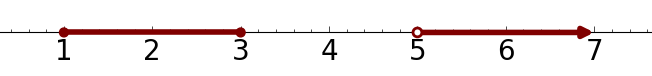
\includegraphics[width=0.5\textwidth]{img/chap1/sec1-2/ex-1-2-11.png}
\caption{A union of intervals.}
\label{fig:1211}
\end{figure}

\begin{example}
Describe the intervals of values shown in Figure \ref{fig:1211} using inequalities and using interval notation.

\begin{solution} To describe the values, $x$, that lie in the intervals shown above
we would say, ``$x$ is a real number greater than or equal to 1 and
less than or equal to 3, or a real number greater than 5.''

As an inequality it is: $1\le x\le 3$ or $x > 5$.

In interval notation: $[1, 3]\cup(5, \infty)$.
\end{solution}\end{example}

\begin{example}
Find the domain of each function.
\begin{itemize}
    \item[(a)] $f(x) = 2\sqrt{x+4}$

    \begin{solution} Since we cannot evaluate the square root of a negative number, we need the inside of the square root to be non-negative. $x+4 \ge 0$ when $x \ge -4$. (Subtract 4 from both sides of the inequality.) Therefore, the domain of $f(x)$ is $[-4, \infty)$.
        \end{solution}
    \item[(b)] $g(x) = \frac{3}{6-3x}$

    \begin{solution} We cannot divide by zero, so we need the denominator to be non-zero. Solving $6-3x = 0$ for $x$, we have $x = 2$, so we must exclude 2 from the domain. Therefore, the domain of $g(x)$ is $(-\infty, 2)\cup(2, \infty)$.
        \end{solution}
\end{itemize}

\end{example}


\subsection{Exercises}
\label{1-2-exercises}

\begin{enumerate}
\item The amount of garbage, $G$, produced by a city with population
  $p$ is given by $G=f(p)$. $G$ is measured in tons per week, and
  $p$ is measured in thousands of people.

  \begin{enumerate}
  \item The town of Tola has a population of 40,000 and produces 13 tons of
    garbage each week. Express this information in terms of the function
    $f$.
  \item Explain the meaning of the statement $f(5)=2$.
  \end{enumerate}

\item The number of cubic yards of dirt, $D$, needed to cover a garden
  with area $a$ square feet is given by $D=g(a)$.

  \begin{enumerate}
  \item A garden with area 5000 ft\textsuperscript{2} requires 50 cubic
    yards of dirt. Express this information in terms of the function
    $g$.
  \item Explain the meaning of the statement $g(100)=1$.
  \end{enumerate}

\item Let $n(t)$ be the number of subscribers to a YouTube channel $t$ years after 2005.
  Explain the meaning of each statement.
  \begin{enumerate}
    \item $n(5) = 300$
    \item $n(10) = 4000$
\end{enumerate}

\item
  Let $p(t)$ be the stock price, in dollars, of Valvoline (VVV) $t$ years after its Initial Public Offering (IPO) on September 23, 2016. Explain the meaning of each statement.
  \begin{enumerate}
    \item $p(0) = 23.10$
    \item $p(1) = 23.27$
    \item $p(2) = 21.47$
\end{enumerate}

\item  Select all of the following graphs which represent $y$ as a function of $x$.

\begin{center}
\begin{tabular}{ccc}
Graph A. & Graph B. & Graph C. \\
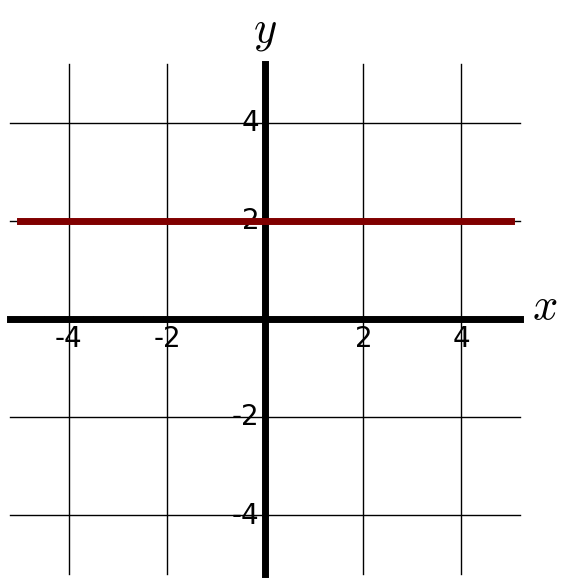
\includegraphics[width=0.2\textwidth]{img/chap1/sec1-2/prob3a.png} & 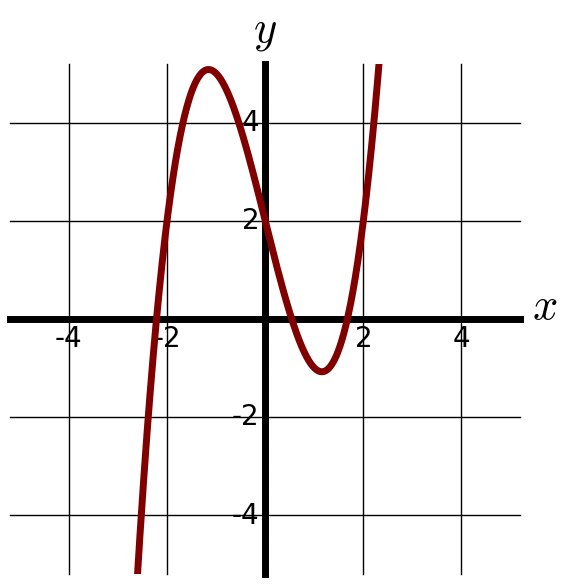
\includegraphics[width=0.2\textwidth]{img/chap1/sec1-2/prob3b.png} &
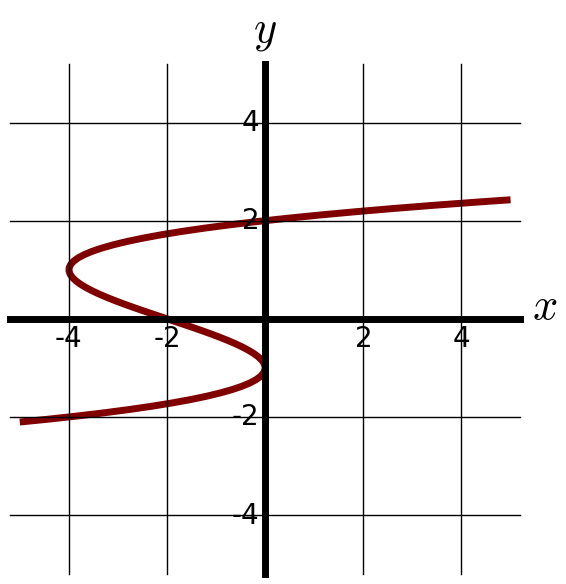
\includegraphics[width=0.2\textwidth]{img/chap1/sec1-2/prob3c.png} \\
\midrule
Graph D. & Graph E. & Graph F. \\
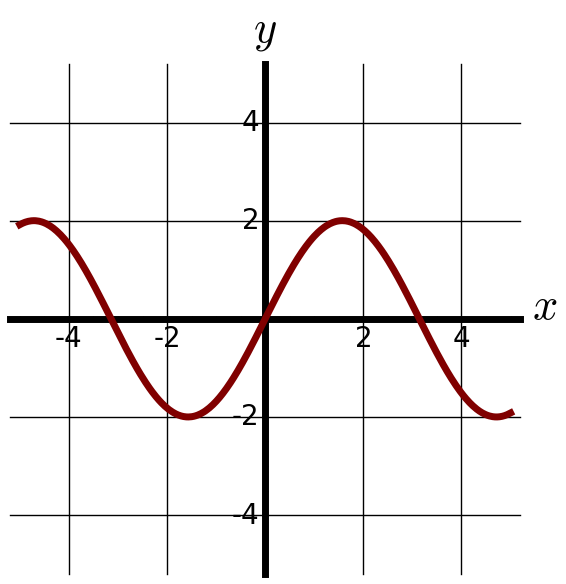
\includegraphics[width=0.2\textwidth]{img/chap1/sec1-2/prob3d.png} & 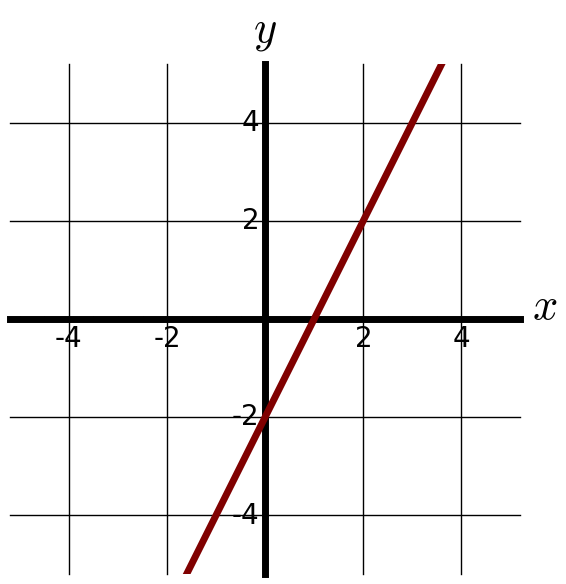
\includegraphics[width=0.2\textwidth]{img/chap1/sec1-2/prob3e.png} &
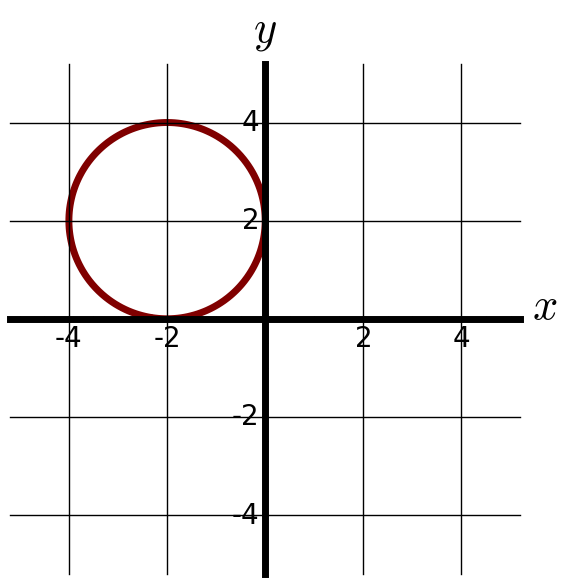
\includegraphics[width=0.2\textwidth]{img/chap1/sec1-2/prob3f.png} \\
\end{tabular}
\end{center}

\item  Select all of the following graphs which represent $y$ as a function of $x$.

\begin{center}
\begin{tabular}{ccc}
Graph A. & Graph B. & Graph C. \\
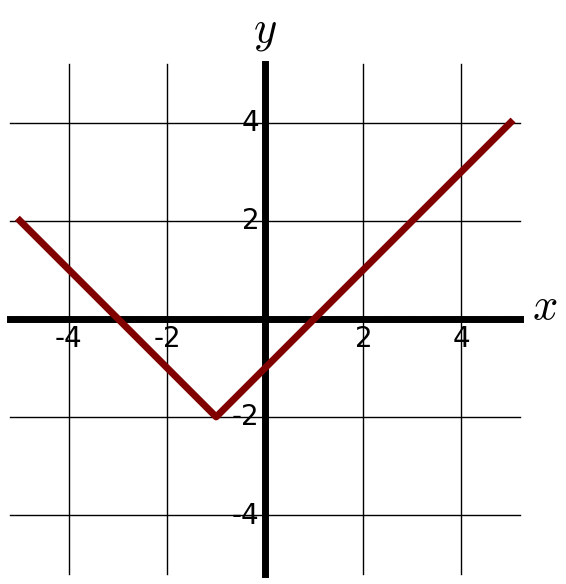
\includegraphics[width=0.2\textwidth]{img/chap1/sec1-2/prob4a.png} & 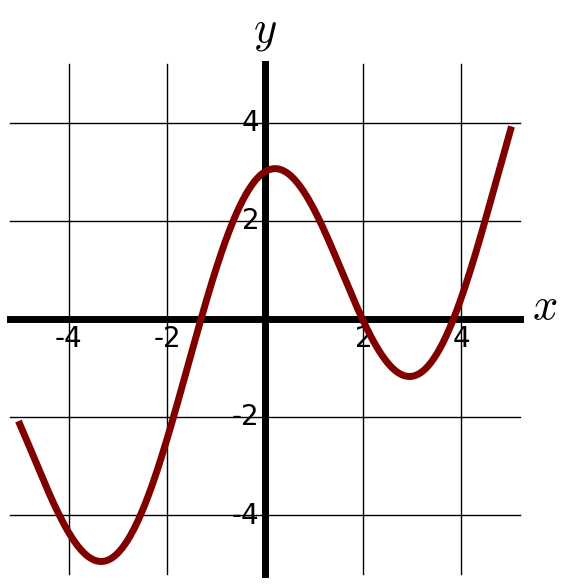
\includegraphics[width=0.2\textwidth]{img/chap1/sec1-2/prob4b.png} &
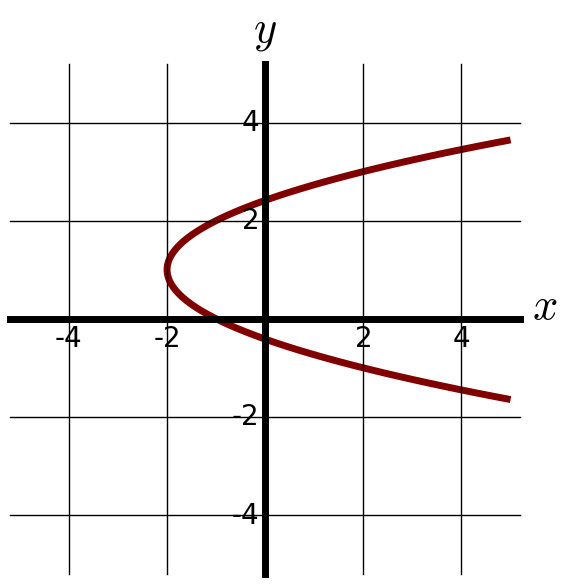
\includegraphics[width=0.2\textwidth]{img/chap1/sec1-2/prob4c.png} \\
\midrule
Graph D. & Graph E. & Graph F. \\
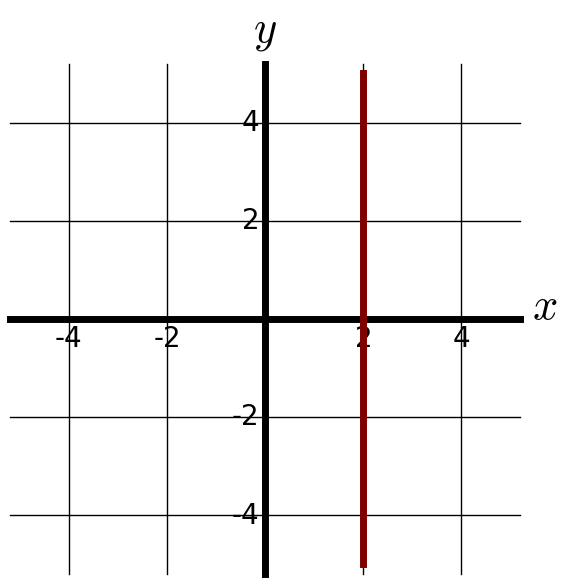
\includegraphics[width=0.2\textwidth]{img/chap1/sec1-2/prob4d.png} & 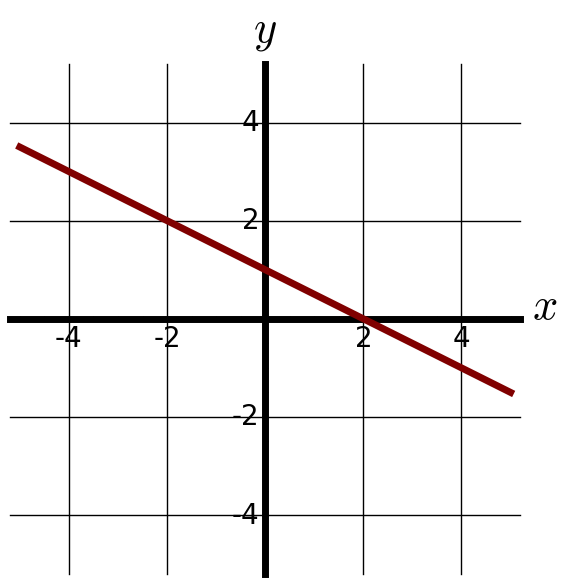
\includegraphics[width=0.2\textwidth]{img/chap1/sec1-2/prob4e.png} &
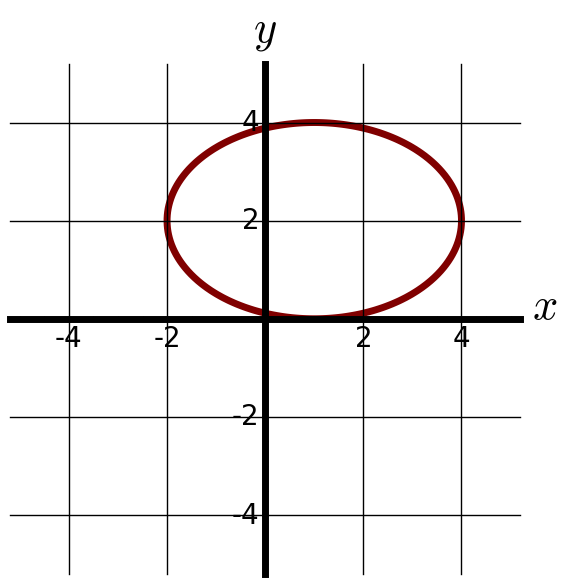
\includegraphics[width=0.2\textwidth]{img/chap1/sec1-2/prob4f.png} \\
\end{tabular}
\end{center}

\item Select all of the following tables which represent $y$ as a function of $x$.
\begin{center}
\begin{tabular}{ccc}
\begin{tabular}{rrrr}
\multicolumn{4}{c}{Table A.}\tabularnewline
\toprule
$x$ & 5 & 10 & 15\tabularnewline
\midrule
$y$ & 3 & 8 & 14\tabularnewline
\bottomrule
\end{tabular}
&
\begin{tabular}{rrrr}
\multicolumn{4}{c}{Table B.}\tabularnewline
\toprule
$x$ & 5 & 10 & 15\tabularnewline
\midrule
$y$ & 3 & 8 & 8\tabularnewline
\bottomrule
\end{tabular}
&
\begin{tabular}{rrrr}
\multicolumn{4}{c}{Table C.}\tabularnewline
\toprule
$x$ & 5 & 10 & 10\tabularnewline
\midrule
$y$ & 3 & 8 & 14\tabularnewline
\bottomrule
\end{tabular}
\end{tabular}
\end{center}

\item Select all of the following tables which represent $y$ as a function of $x$.
\begin{center}
\begin{tabular}{ccc}
\begin{tabular}{rrrr}
\multicolumn{4}{c}{Table A.}\tabularnewline
\toprule
$x$ & 2 & 6 & 13\tabularnewline
\midrule
$y$ & 3 & 10 & 10\tabularnewline
\bottomrule
\end{tabular}
&
\begin{tabular}{rrrr}
\multicolumn{4}{c}{Table B.}\tabularnewline
\toprule
$x$ & 2 & 6 & 6\tabularnewline
\midrule
$y$ & 3 & 10 & 14\tabularnewline
\bottomrule
\end{tabular}
&
\begin{tabular}{rrrr}
\multicolumn{4}{c}{Table C.}\tabularnewline
\toprule
$x$ & 2 & 6 & 13\tabularnewline
\midrule
$y$ & 3 & 10 & 14\tabularnewline
\bottomrule
\end{tabular}
\end{tabular}
\end{center}

\item Select all of the following tables which represent $y$ as a function of $x$.
\begin{center}
\begin{tabular}{cccc}
\begin{tabular}{rr}
\multicolumn{2}{c}{Table A.}\tabularnewline
\toprule
$x$ & $y$\tabularnewline
\midrule
0 & $-2$\tabularnewline
3 & 1\tabularnewline
4 & 6\tabularnewline
8 & 9\tabularnewline
3 & 1\tabularnewline
\bottomrule
\end{tabular}
&
\begin{tabular}{rr}
\multicolumn{2}{c}{Table B.}\tabularnewline
\toprule
$x$ & $y$\tabularnewline
\midrule
$-1$ & $-4$\tabularnewline
2 & 3\tabularnewline
5 & 4\tabularnewline
8 & 7\tabularnewline
12 & 11\tabularnewline
\bottomrule
\end{tabular}
&
\begin{tabular}{rr}
\multicolumn{2}{c}{Table C.}\tabularnewline
\toprule
$x$ & $y$\tabularnewline
\midrule
0 & $-5$\tabularnewline
3 & 1\tabularnewline
3 & 4\tabularnewline
9 & 8\tabularnewline
16 & 13\tabularnewline
\bottomrule
\end{tabular}
&
\begin{tabular}{rr}
\multicolumn{2}{c}{Table D.}\tabularnewline
\toprule
$x$ & $y$\tabularnewline
\midrule
$-1$ & $-4$\tabularnewline
1 & 2\tabularnewline
4 & 2\tabularnewline
9 & 7\tabularnewline
12 & 13\tabularnewline
\bottomrule
\end{tabular}
\end{tabular}
\end{center}

\item Select all of the following tables which represent $y$ as a function of $x$.

\begin{center}
\begin{tabular}{cccc}
\begin{tabular}{rr}
\multicolumn{2}{c}{Table A.}\tabularnewline
\toprule
$x$ & $y$\tabularnewline
\midrule
$-4$ & $-2$\tabularnewline
3 & 2\tabularnewline
6 & 4\tabularnewline
9 & 7\tabularnewline
12 & 16\tabularnewline
\bottomrule
\end{tabular}
&
\begin{tabular}{rr}
\multicolumn{2}{c}{Table B.}\tabularnewline
\toprule
$x$ & $y$\tabularnewline
\midrule
$-5$ & $-3$\tabularnewline
2 & 1\tabularnewline
2 & 4\tabularnewline
7 & 9\tabularnewline
11 & 10\tabularnewline
\bottomrule
\end{tabular}
&
\begin{tabular}{rr}
\multicolumn{2}{c}{Table C.}\tabularnewline
\toprule
$x$ & $y$\tabularnewline
\midrule
$-1$ & $-3$\tabularnewline
1 & 2\tabularnewline
5 & 4\tabularnewline
9 & 8\tabularnewline
1 & 2\tabularnewline
\bottomrule
\end{tabular}
&
\begin{tabular}{rr}
\multicolumn{2}{c}{Table D.}\tabularnewline
\toprule
$x$ & $y$\tabularnewline
\midrule
$-1$ & $-5$\tabularnewline
3 & 1\tabularnewline
5 & 1\tabularnewline
8 & 7\tabularnewline
14 & 12\tabularnewline
\bottomrule
\end{tabular}
\end{tabular}
\end{center}

\begin{minipage}{\linewidth}
\begin{wrapfigure}{r}{0.4\textwidth}
    \centering
    \vspace{-12pt}
    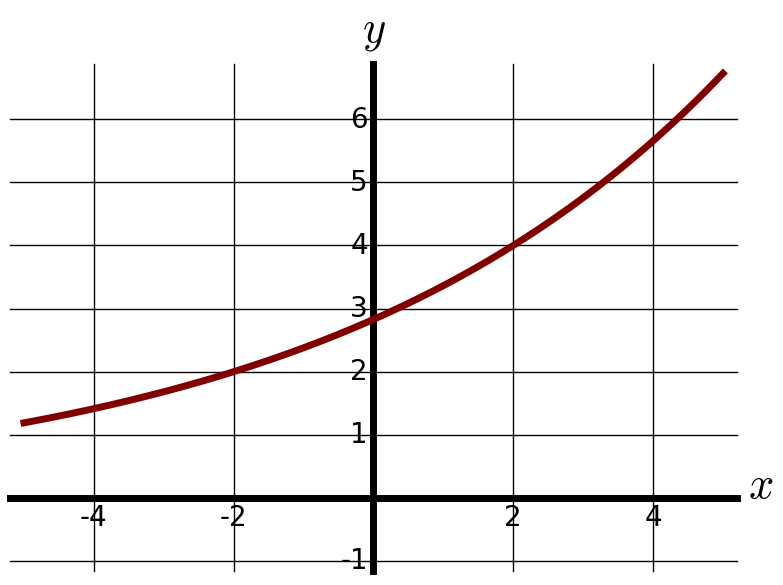
\includegraphics[width=0.4\textwidth]{img/chap1/sec1-2/prob7.png}
\end{wrapfigure}

\item Let $g(x)$ be the function graphed on the right.
    \begin{enumerate}
        \item Evaluate $g(2)$.
        \item Solve $g(x) = 2$ for $x$.
    \end{enumerate}
\end{minipage}

\vspace{120pt}

\begin{minipage}{\linewidth}
\begin{wrapfigure}{r}{0.4\textwidth}
    \centering
    \vspace{-36pt}
    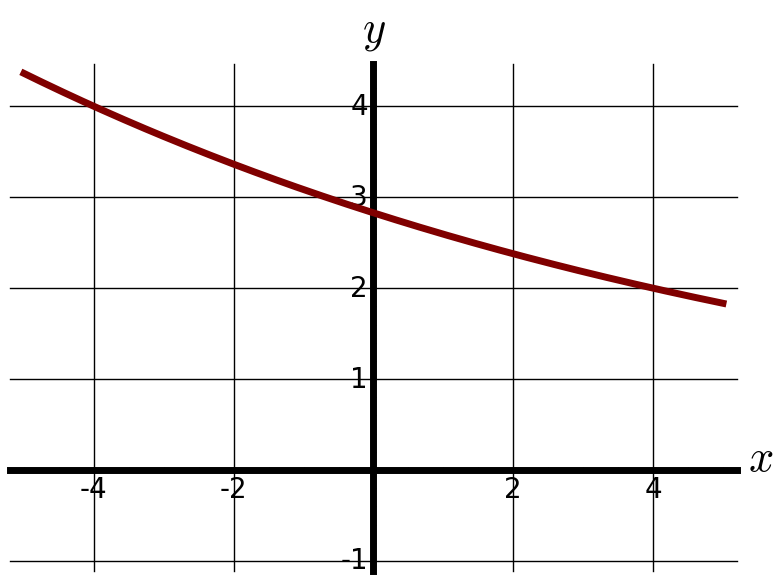
\includegraphics[width=0.4\textwidth]{img/chap1/sec1-2/prob8.png}
\end{wrapfigure}

\item Let $f(x)$ be the function graphed on the right.
    \begin{enumerate}
        \item Evaluate $f(4)$.
        \item Solve $f(x) = 4$ for $x$.
    \end{enumerate}
\end{minipage}


\vspace{120pt}

\begin{minipage}{\linewidth}
\begin{wraptable}{r}{0.6\textwidth}
    \centering
    \vspace{-12pt}
    \begin{longtable}[]{@{}lrrrrrrrrrr@{}}
    \toprule
    $x$ & 0 & 1 & 2 & 3 & 4 & 5 & 6 & 7 & 8 & 9\tabularnewline
    \midrule
    \endhead
    $f(x)$ & 74 & 28 & 1 & 53 & 56 & 3 & 36 & 45 & 14 & 47\tabularnewline
    \bottomrule
    \end{longtable}
\end{wraptable}

\item Consider the table at right.
    \begin{enumerate}
        \item Evaluate $f(3)$.
        \item Solve $f(x) = 1$ for $x$.
    \end{enumerate}
\end{minipage}

\begin{minipage}{\linewidth}
\begin{wraptable}{r}{0.6\textwidth}
    \centering
    \vspace{-12pt}
    \begin{longtable}[]{@{}lrrrrrrrrrr@{}}
    \toprule
    $x$ & 0 & 1 & 2 & 3 & 4 & 5 & 6 & 7 & 8 & 9\tabularnewline
    \midrule
    \endhead
    $g(x)$ & 62 & 8 & 7 & 38 & 86 & 73 & 70 & 39 & 75 & 34\tabularnewline
    \bottomrule
    \end{longtable}
\end{wraptable}

\item  Consider the table at right.
\begin{enumerate}
    \item Evaluate $g(8)$.
    \item Solve $g(x) = 7$ for $x$.
\end{enumerate}
\end{minipage}

\vspace{24pt}

\noindent For Exercises 15-22, evaluate: $f(-2)$, $f(-1)$, $f(0)$, $f(1)$, and $f(2)$, if possible.

\item $f(x) = 4 - 2 x$
\item $f(x) = 8-3x$
\item $f(x) = 8x^2 - 7x + 3$
\item $f(x) = 6x^2 - 7x + 4$
\item $f(x) = 3 + \sqrt{x+3}$
\item $f(x) = 4 - \sqrt[3]{x-2}$
\item $f(x) = \frac{x-3}{x+1}$
\item $f(x) = \frac{x-2}{x+2}$

\item Let $f(t) = 3t+5$.
\begin{enumerate}
    \item Evaluate $f(0)$.
    \item Solve $f(t) = 0$ for $t$.
\end{enumerate}

\item Let $g(p) = 6-2p$.
\begin{enumerate}
    \item Evaluate $g(0)$.
    \item Solve $g(p) = 0$ for $t$.
\end{enumerate}

\begin{minipage}{\linewidth}
\begin{wrapfigure}{r}{0.5\textwidth}
    \centering
    \vspace{-100pt}
    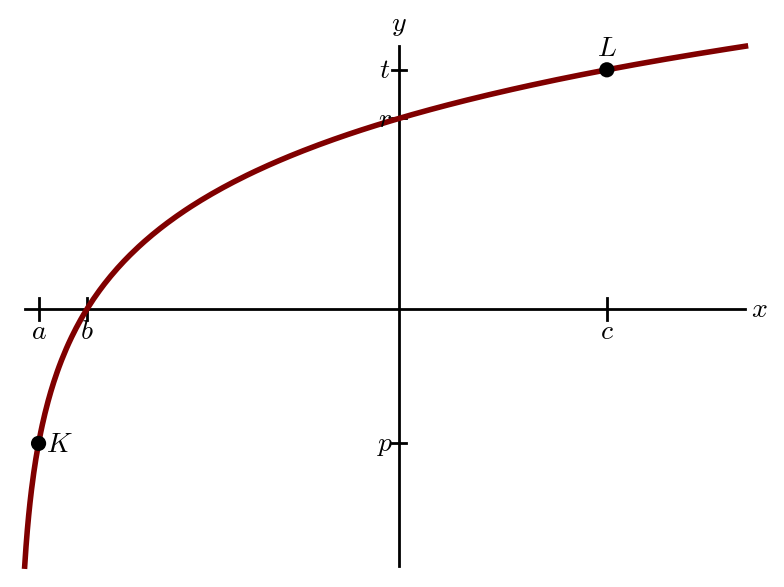
\includegraphics[width=0.48\textwidth]{img/chap1/sec1-2/prob21.png}
\end{wrapfigure}
\item Consider the graph of $f(x)$ on the right.
    \begin{enumerate}
        \item Evaluate $f(c)$.
        \item Solve $f(x) = p$ for $x$.
        \item Find the coordinates of points $L$ and $K$.
    \end{enumerate}
\end{minipage}
\end{enumerate}
